\section{Spatial Features}
\label{chp:spatial}
Considering only one POI's location, it can be as simple as a pair longitude and latitude.
However, with relative position with each other, more information emerges.
Such information is closely related to the POI's functional characteristics,
which indicate their categories. POIs with different categories show different
characteristics on many statistics related to spatial aspects as explained
following in details, and thus different features work well on different
categories. In the following, we analyze different kinds of spatial features
on part of New York data crawled from Foursquare.
We consider only the first level categories for simplicity,
because the same features can be applied to the second level categories
(shown in experiments).

\subsection{Neighborhood Category Distribution}
%\begin{figure}[ht]
%\begin{minipage}{0.5\linewidth}
%\centering
%\includegraphics[width=\columnwidth]{plot/No_other_POI_within_100m.eps}
%\caption{No other POIs within 100m}
%\label{fig:NoPOI}
%\end{minipage}
%\hspace{0.5cm}
%\begin{minipage}{0.5\linewidth}
%\centering
%\includegraphics[width=\columnwidth]{plot/Shop_and_Service_and_Professional_and_Other_Places_neighbor_within_100m.eps}
%\caption{Shop \& Service's and Professional \& Other Places 's neighbor within 100m}
%\label{fig:ShopProf}
%\end{minipage}
%\end{figure}


We observe that POIs related to each other often appear in the same zone.
For example, a shopping center has shops and restaurants, a financial center
has banks and office buildings, or a college town has colleges, museums,
and observatories. Neighborhood shows functionality of an area and thus
provides a prior probability of the category a POI may belong to. In addition,
since different categories show great difference in their neighborhood composition,
neighbourhood profile is also good at differentiating POIs in different categories.

As shown in Figure \ref{fig:NoPOI}, according to our analysis on POIs in New York
from Foursquare data, around 30\% of ``Outdoors \& Recreation'' have no other POIs
near them within 100 meters, indicating their ``isolation'', while most of ``Food'' have
other POIs near them, indicating a symbiotic relationship of ``Food'' with other
interesting spot. The reason is that people often visit a restaurant when 
they are on the way to or leaving some POIs like shops, cinemas, etc.  
%The fact is reasonable since ``Food'' relies on customers visiting,
%however most of restaurants are not attractive enough for people to go there on purpose,
%so they have to bound with places attracting people. \KQ{Don't understand this sentence.
%You mean most of the restaurants are in downtown? should be not attractive enough
%for people to travel a long distance to get there?}
On the contrary, POIs in
``Outdoors \& Recreation'' are usually built in a
large space, thus suburban would be a wise choice. From the figure we can also
see that ``Nightlife Spot'', ``Shop \& Service'' are often around with other POIs,
too, which also gets along with common sense.

Not only the ``crowding'' within a POI's neighborhood differs from one category to another,
the category distribution of the neighborhood also differs from one to another.
Firstly, we should notice that there exists some extreme cases in category
distribution, such as ``Food'' is everywhere while there's very few ``college''
near most of POIs in the city. However, difference still stands out between categories.
As shown in the Figure \ref{fig:ShopProf} we can see there are more food and shops
around ``Shop \& Service'', but there are more ``College \& University'',
``Professional \& Other Places'' near ``College \& University''.
%\begin{figure}[ht]
%\begin{minipage}{0.45\linewidth}
%\centering
%\includegraphics[width=\columnwidth]{plot/F1_measure_using_NB_100_feature.eps}
%\caption{F1 measure using NB\_100m feature}
%\label{fig:F1NB100}
%\end{minipage}
%\begin{minipage}{0.55\linewidth}
%\centering
%\includegraphics[width=\columnwidth]{plot/F1_measure_using_NB_m_feature_on_Shop_and_Service_and_Residence.eps}
%\caption{F1 measure using NB\_m feature on Shop \& Service and Residence with different m}
%\label{fig:F1NBShopResi}
%\end{minipage}
%\end{figure}

Therefore, we introduce NB\_m feature to describe the category distributions
within certain distance around the POI. The NB\_m feature is defined as:
for a POI $i$, the category distribution of all the POIs
within $i$'s m meters and the number of POIs within m meters.

%To prove NB\_m feature's effectiveness, we set $m = 100$ and add NB\_100 feature to BASE feature and test on all categories, it yields better classification result for all as shown in figure \ref{fig:F1NB100}.
%
%Furthermore, with further testing, it appears that different m should be set for different categories. We test on different $m = 10,50,100$, and they result in different performances. Take ``Residence'' and ``Shop \& Service'' as example, as shown in Figure \ref{fig:F1NBShopResi}, NB\_10 yields best result for ``Residence'', and larger m would lower the score, however, ``Shop \& Service'' prefer larger m, and it gains best result when m equals 100.

\begin{figure}
  \centering
  \begin{minipage}[b]{.4\linewidth}
    \centering
    \includegraphics[width=\columnwidth]{plot/No_other_POI_within_100m.eps}
  \end{minipage}%
  %\hspace{-0.75cm}
  \begin{minipage}[b]{.6\linewidth}
    \centering
    %\includegraphics[width=\columnwidth]{plot/Shop_and_Service_and_Professional_and_Other_Places_neighbor_within_100m.eps}
    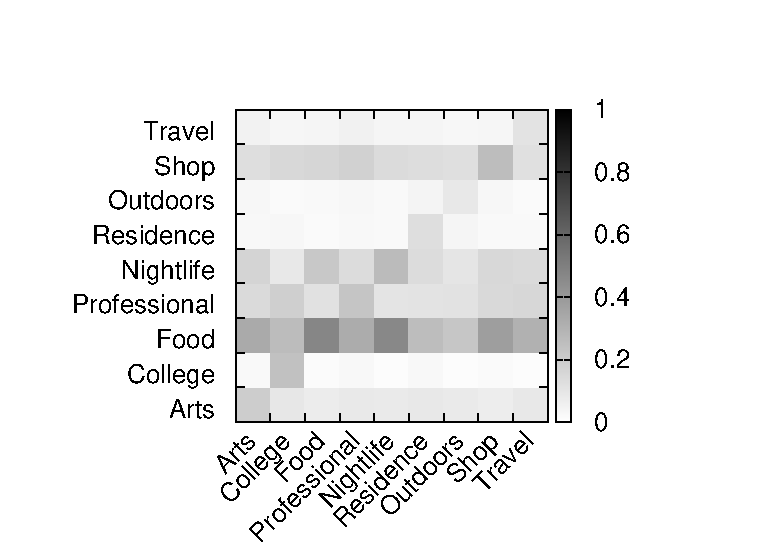
\includegraphics[width=\columnwidth]{plot/ColorMap/Shop_and_Service_and_Professional_and_Other_Places_neighbor_within_100m.eps}
  \end{minipage}\\%[-10pt]

  \begin{minipage}[t]{.4\linewidth}
    \caption{No other POIs within 100m}
    \label{fig:NoPOI}
  \end{minipage}%
  \hspace{0.3cm}
  \begin{minipage}[t]{.55\linewidth}
    %\caption{Shop \& Service's and Professional \& Other Places 's neighbor within 100m}
    \caption{Different categories'(xtics) category distribution(ytics) within 100m}
    \label{fig:ShopProf}
  \end{minipage}%
\end{figure}

\subsection{ The Nearest K POIs}
%\begin{figure}[ht]
%\begin{minipage}[ht]{0.5\linewidth}
%\centering
%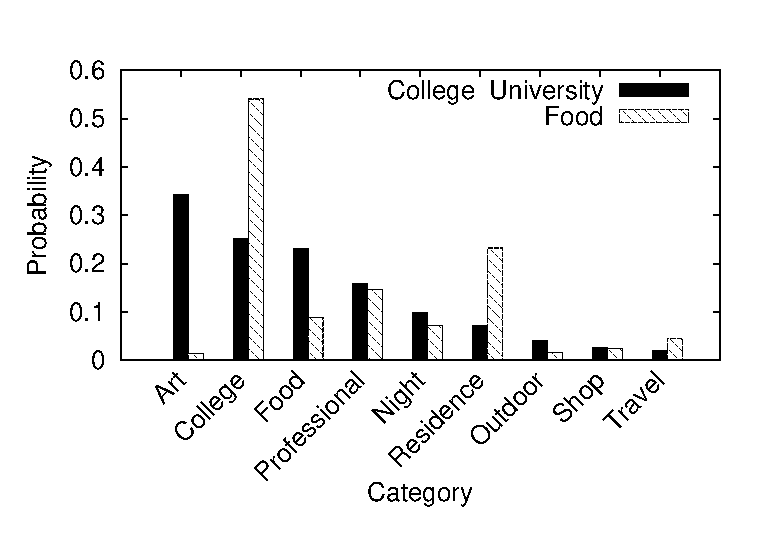
\includegraphics[width=\columnwidth]{plot/Food_and_College_1-Nearest_POI_category_distribution.eps}
%\caption{Food's \& College's 1-Nearest POI category distribution}
%\label{fig:foodcollege}
%\end{minipage}
%\begin{minipage}[ht]{0.5\linewidth}
%\centering
%\includegraphics[width=\columnwidth]{plot/F1_measure_using_N_5_feature.eps}
%\caption{F1 measure using N\_5 feature}
%\label{fig:F1N5}
%\end{minipage}
%\end{figure}


Apart from neighborhood functionality, we find the nearest $k$ POIs'
category as another feature to compensate the NB\_m feature.
It is because the NB\_m feature represents the general
functionality in a big area, but there are often some
concentrations on specific spots. As showed in Figure \ref{fig:foodcollege},
``Food'' and ``College \& University'' show typical intention
aggregating on some spots. For ``College \& University'', no matter
they locate in urban or suburban, the college buildings are definitely
close to each other. And for ``Food'', we can see the trend very often
in our life: there might be a street of local snack, or a part of
business zone full of restaurants. Besides that, other than similar POIs
aggregating together, some categories instinctively near together.
For example, ``Nightlife Spot'' are often mixed with ``Food'',
which is another typical characteristic for both ``Nightlife Spot'' and ``Food''.

It seems that the nearest $k$ POIs feature is a part of POI's neighborhood feature.
However, focusing on the nearest POIs gives extra information on the particular spot the POI is on.
For example, although the neighborhood mainly consists of office buildings,
if the target POI lies in a part of the region that is full of restaurants,
it is more possible that the POI belongs to ``Food''.
In other words, POI's neighborhood is considering a neighborhood based on
the absolute distance, which not only represents the neighborhood's attribute,
but also tells how bustling within the region.
The nearest $k$ POIs feature is a relative neighborhood which considers
only the nearest $k$ POIs, no matter they are far away from each other
or very close to each other. In fact, the two kinds of feature do show
big difference in experiment and we cannot replace one to another.

We use N\_k to abbreviate the nearest k POIs' category distribution.
The N\_k feature is defined as: for a POI i, the category distribution of nearest $k$ POIs within 1km to $i$.

%We further test the influence of selection of k on the result setting $k=1,5,10,20$. According to our experiment, having larger k won't change result very much, we show ``Food'' and ``Nightlife Spot'' as example in Figure \ref{fig:F1NKFoodNight}. However, as we will discuss more in Chapter \ref{Experiment}, since different m in NB\_m will differ very much in result and different m combining different k in N\_k feature will also results in different result, accordingly different k will be needed in final feature construction for different categories.


%{\centering
%\begin{minipage}[ht]{0.5\linewidth}
%\centering
%\includegraphics[width=\columnwidth]{plot/F1_measure_using_N_K_feature_on_Food_and_Nightlife_Spot.eps}
%\captionof{figure}{F1 measure using N\_K feature on Food and Nightlife Spot with different K}
%\label{fig:F1NKFoodNight}
%\end{minipage}
%\begin{minipage}{0.49\linewidth}
%  \centering
%  \small
%  \begin{tabular}{ll}
%
%  \hline\noalign{\smallskip}
%  Category & Distance(m)  \\
%  \noalign{\smallskip}\hline\noalign{\smallskip}
%  Professional \& Other Places  &    210.851 \\
%  Nightlife Spot  &   227.3833 \\
%  Shop \& Service  &   227.5524 \\
%  Arts \& Entertainment  &   230.5648 \\
%  Food  &   237.8074 \\
%  College \& University  &    275.849 \\
%  Residence  &   308.1981 \\
%  \noalign{\smallskip}\hline
%  \end{tabular}
%  \captionof{table}{Different categories' average distance to nearest ``Travel and Transport''}
%  \label{tab:DisToTravel}
%\end{minipage}
%
%}



\begin{figure}[ht]
\centering
%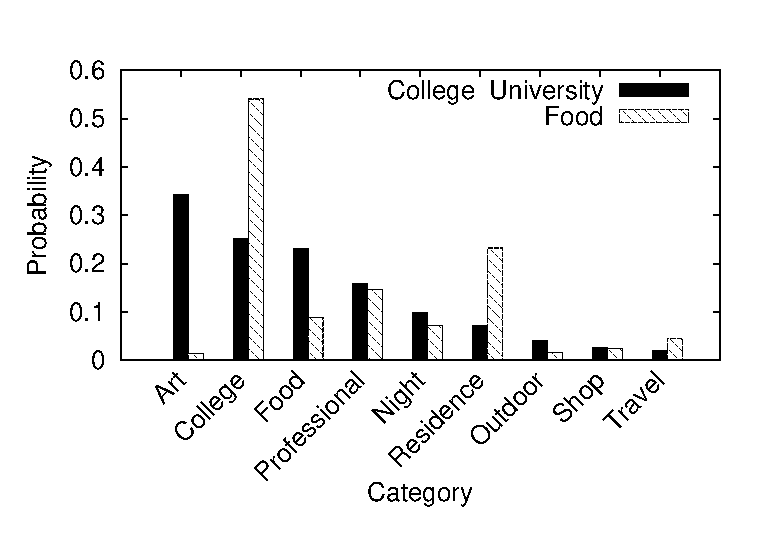
\includegraphics[width=0.7\columnwidth]{plot/Food_and_College_1-Nearest_POI_category_distribution.eps}
\includegraphics[width=0.8\columnwidth]{plot/ColorMap/Food_and_College_1-Nearest_POI_category_distribution.eps}
\caption{Food's \& College's 1-Nearest POI category distribution}
\label{fig:foodcollege}
\end{figure}

\subsection{ Distance to Category}
\label{sec:lcd}
The NB\_m and N\_k feature are insufficient to identify the category for a
POI in some cases. For example, if a POI is located close to a lot of restaurants,
then the POI is supposed to be in category ``Food'' according to the NB\_m and N\_k features.
However, if the POI is far from ``Shop \& Services''
and ``Art \& Entertainments'', then the
POI is probably not a restaurant but a residence.
Due to this fact, we also examine the influence of category
distance, which is the distance from the target POI to
the nearest POI in each category.
%With the NB\_m feature and N\_k feature above, we have a good representation
%for the POIs near the target POI. However, we haven't considered those POIs
%which are not in $m$ meters in NB\_m, and not in the top $k$ list in N\_k.
%There's also a reason why those POIs are, in some sense, far away from the target POI.
%So in order to extract valid information from the POIs that are not near,
%we utilize the feature that shows the distance to the nearest POI in different
%categories, and it exhibits more characteristics. For example, from above
%features including NB\_m and N\_k, a POI shows that it is located close to
%``Food'', based on these, the POI belonging to ``Food'' is a reasonable
%prediction. However, if distance to categories feature tell us more that the
%POI is far from ``Shop \& Services'' and ``Art \& Entertainments'', then the
%probability of the POI belonging to ``Residence'' also rise up.
%We found some interesting facts about category distance.
Specifically, we first examine different categories' average distance
to nearest ``Travel and Transport'' to see which categories are often
near transportation. We show the distances in Table \ref{tab:DisToTravel},
and we find that ``Professional \& Other Places'' is the nearest to transportation,
which is quite reasonable since otherwise the cooperation need to run regular bus for its employees.

\begin{table}[ht]
\centering
%\small
% table caption is above the table
\caption{Different categories' average distance to nearest ��Travel and Transport��}
\label{tab:DisToTravel}       % Give a unique label
% For LaTeX tables use
\begin{tabular}{llll}
\hline\noalign{\smallskip}
Category & Distance(m) &Category & Distance(m) \\
\noalign{\smallskip}\hline\noalign{\smallskip}
Professional \& Other Places  &    \textbf{210.851} &   College \& University  &    275.849   \\
Nightlife Spot  &   227.3833 &Residence  &   308.1981 \\
Shop \& Service  &   227.5524 &Travel \& Transport  & 9788.035\\
Arts \& Entertainment  &   230.5648 &  Outdoors \& Recreation & 12272.19\\
 Food  &   237.8074 & & \\
\noalign{\smallskip}\hline
\end{tabular}
\end{table}

Then, we examine the distance of each category to all other categories in Figure \ref{fig:LogCD}.
From the figure, we observe that ``Outdoor \& Recreation'' is far from all categories,
while ``Food'' is near to all.
This fact gets along with our analysis in Figure \ref{fig:NoPOI} that
there's very few POIs near ``Outdoor'', but ``Food'' can be found everywhere.

Formally, we define the category distance feature ($CD$) for a POI $i$ and a category $c$ as:
\begin{equation}
CD_{i,c}= min_{j \in c} distance(i,j).
\end{equation}

The linear definition of category distance is straightforward but not close to
the fact. POIs in 100km from the target POI and those in 200km
have not much difference for identifying the target POI's category because
both of them are too \emph{far}. In contrast, the classifier should be sensitive
to the difference between two short distances. Therefore, we propose two
variations to $CD$, i.e., $LCD1, LCD2$ as follows:
\begin{align}
LCD1_{i,c} &= \log{(1+CD_{i,c})},\\
LCD2_{i,c} &= \log{(1+\log{(1+CD_{i,c})})}.
\end{align}



%According to our experiment, directly using $CD$ as features in classification is not effective, and a reasonable process is to take log operation, therefore we further define $LCD1, LCD2$ as, for each POI $i$,
%\begin{align}
%LCD1_i &= Log(1+CD_i)\\
%LCD2_i &= Log(1+ Log(1+CD_i))
%\end{align}


%\begin{figure}
%\begin{minipage}[ht]{0.5\linewidth}
%\centering
%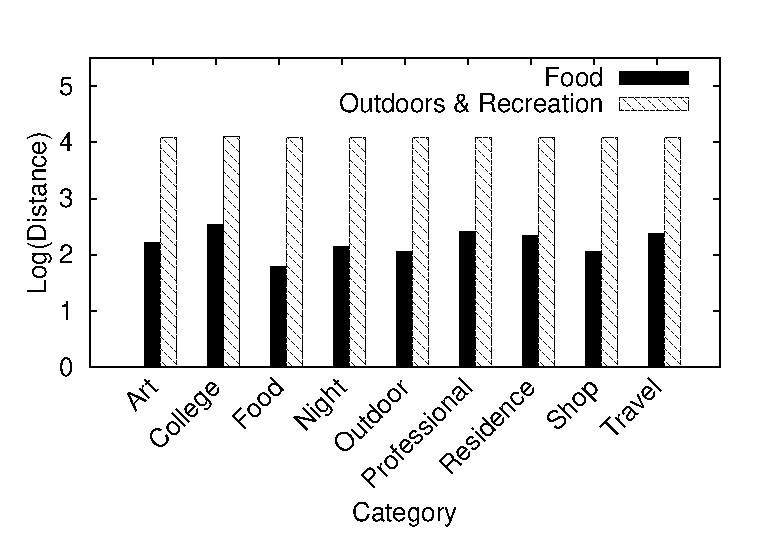
\includegraphics[width=\columnwidth]{plot/LogAvgCD.eps}
%\caption{Log(Avg(Category Distance))}
%\label{fig:LogCD}
%\end{minipage}
%\begin{minipage}{0.5\linewidth}
%  %\centering
%  %\raggedleft
%  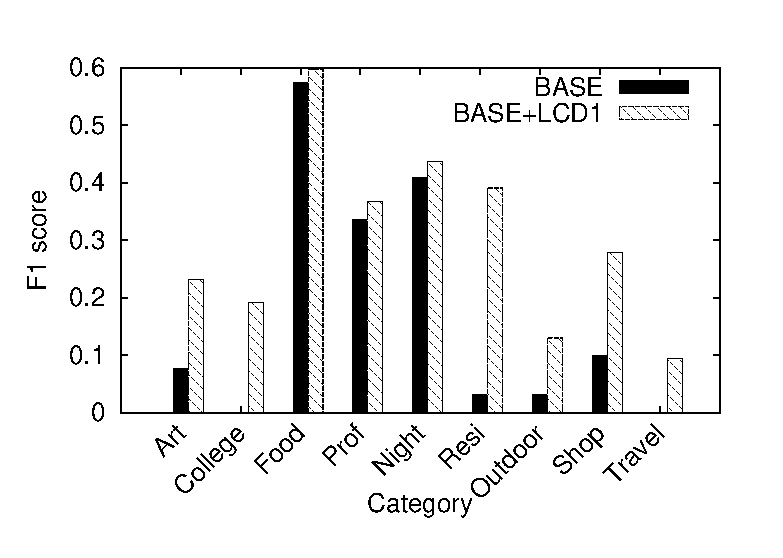
\includegraphics[width=\columnwidth]{plot/F1_measure_using_LCD1_feature.eps}
%  \caption{F1 measure using LCD1 feature}
%  \label{fig:F1LogCD}
%\end{minipage}
%
%\end{figure}

\begin{figure}[ht]
\centering
\includegraphics[width=0.8\columnwidth]{plot/ColorMap/Color_CategoryDis.eps}
%\caption{Log(Avg(Category Distance))}
\caption{Average Category Distance with log operation, darker indicates a larger distance}
\label{fig:LogCD}
\end{figure}

\subsection{ Region Comparison}


%\begin{figure}[ht]
%\centering
%% Use the relevant command to insert your figure file.
%% For example, with the graphicx package use
%  \epsfig{file=plot/F1_measure_using_RegCom_T_feature.eps,width=0.7\columnwidth}
%% figure caption is below the figure
%\caption{F1 measure using RegCom feature}
%\label{fig:F1RC}       % Give a unique label
%\end{figure}
Region Comparison feature aims at comparing the target POI with other POIs within
the same region on the user behaviors. The motivation is that some categories
may often be ``destinations'' of a user's travel activity, such as ``Art \& Entertainment'',
while some categories may often be on the way to the destination, such as ``Food''.
We assume that the places which are more popular (according to users and check-ins) than other places nearby,
is more probable to be a destination. To make use of the user check-in information,
we consider both the number of check-ins and the number of unique users. We compare
the check-ins and unique users of the target POI to the POIs within a distance of m,
and compute the average difference of check-ins and unique users as the
region comparison feature for the POI. The region comparison feature for total
check-ins (RC\_T\_m(i,c)) and for unique users (RC\_U\_m(i,c)) are computed as follows:
%Thus with such feature, we combine
%the factor from both spatial environment and user behavior. As for user behavior,
%inspired by the previous work, we consider the number of check-ins and unique users.
%Therefore, we compare the target POI's number of total check-ins and unique users
%with the POIs around it, and the region is precisely defined by a radius of m.
%In NB\_m, we apply different m to define neighborhood for different categories,
%likewise, we also build several different Region Comparison features with different m.
%In terms of comparison, we do substraction between the average level of user behavior measures and the target POI's digits. Formally, we define $Region Comparison\_Total Check-in (RC\_T\_m)$ and $Region Comparison\_Unique Users (RC\_U\_m)$ as
\begin{equation}
RC\_T\_m(i,c) = Avg_{j \in c, distance(i,j)<m} \#Checkin(j) - \#Checkin(i) 
\label{eq:rct}
\end{equation}
\begin{equation}
RC\_U\_m(i,c) = Avg_{j \in c, distance(i,j)<m} \#UniqueUser(j) - \#UniqueUser(i)
\label{eq:rcu}
\end{equation}

Figure \ref{fig:RC} shows the average region comparison feature of 
total check-ins for the five categories of POIs.
The score below 0 means that people check in more times at target POI than the POIs near it.
%Checking in a place more than the ones near it is actually saying that people are gathered to the place, or in other word, it is a ``destination'', not a ``by the way''.
Intuitively, ``Art \& Entertainment'' is more of a ``destination'', people come in purpose
to watch a show, or see an exhibition. ``Outdoor \& Recreation'' is more of a ``destination'', too,
since people planned beforehand to have a weekend with children on a beach, or have a routine of
going to fishing spot. ``Food'' is a ``on the way'' category both by intuition and statistics.
People grab something to eat all the time: after a walk or before a movie. Interestingly, we
find that ``Shop \& Service'' shows the character of a ``by the way'', too.
It seems interesting shops are growing in number, and consequently people are attracted into a
shop though not intended. In contrast, nightlife spot's are more of destinations, because they 
are usually the last places people may visit in daily life. 
%it seems bars are getting more popularity and loyalty from customers than shops and food.

%To show the strength of region comparison features, we set m to be 100 for both RC\_T\_m and RC\_U\_m, and test the features on the nine first level categories, the result is shown in Figure \ref{fig:F1RC}. When the features are combining with BASE and m set to be 100, RC\_T\_m and RC\_U\_m show similar strength in classification, however, as we will discuss more on experiment in Chapter \ref{Experiment}, RC\_U\_m appears to be more effective than RC\_T\_m. Overall, they do show improvements but not as powerful as previous ones.
\begin{figure}[ht]
% Use the relevant command to insert your figure file.
% For example, with the graphicx package use
  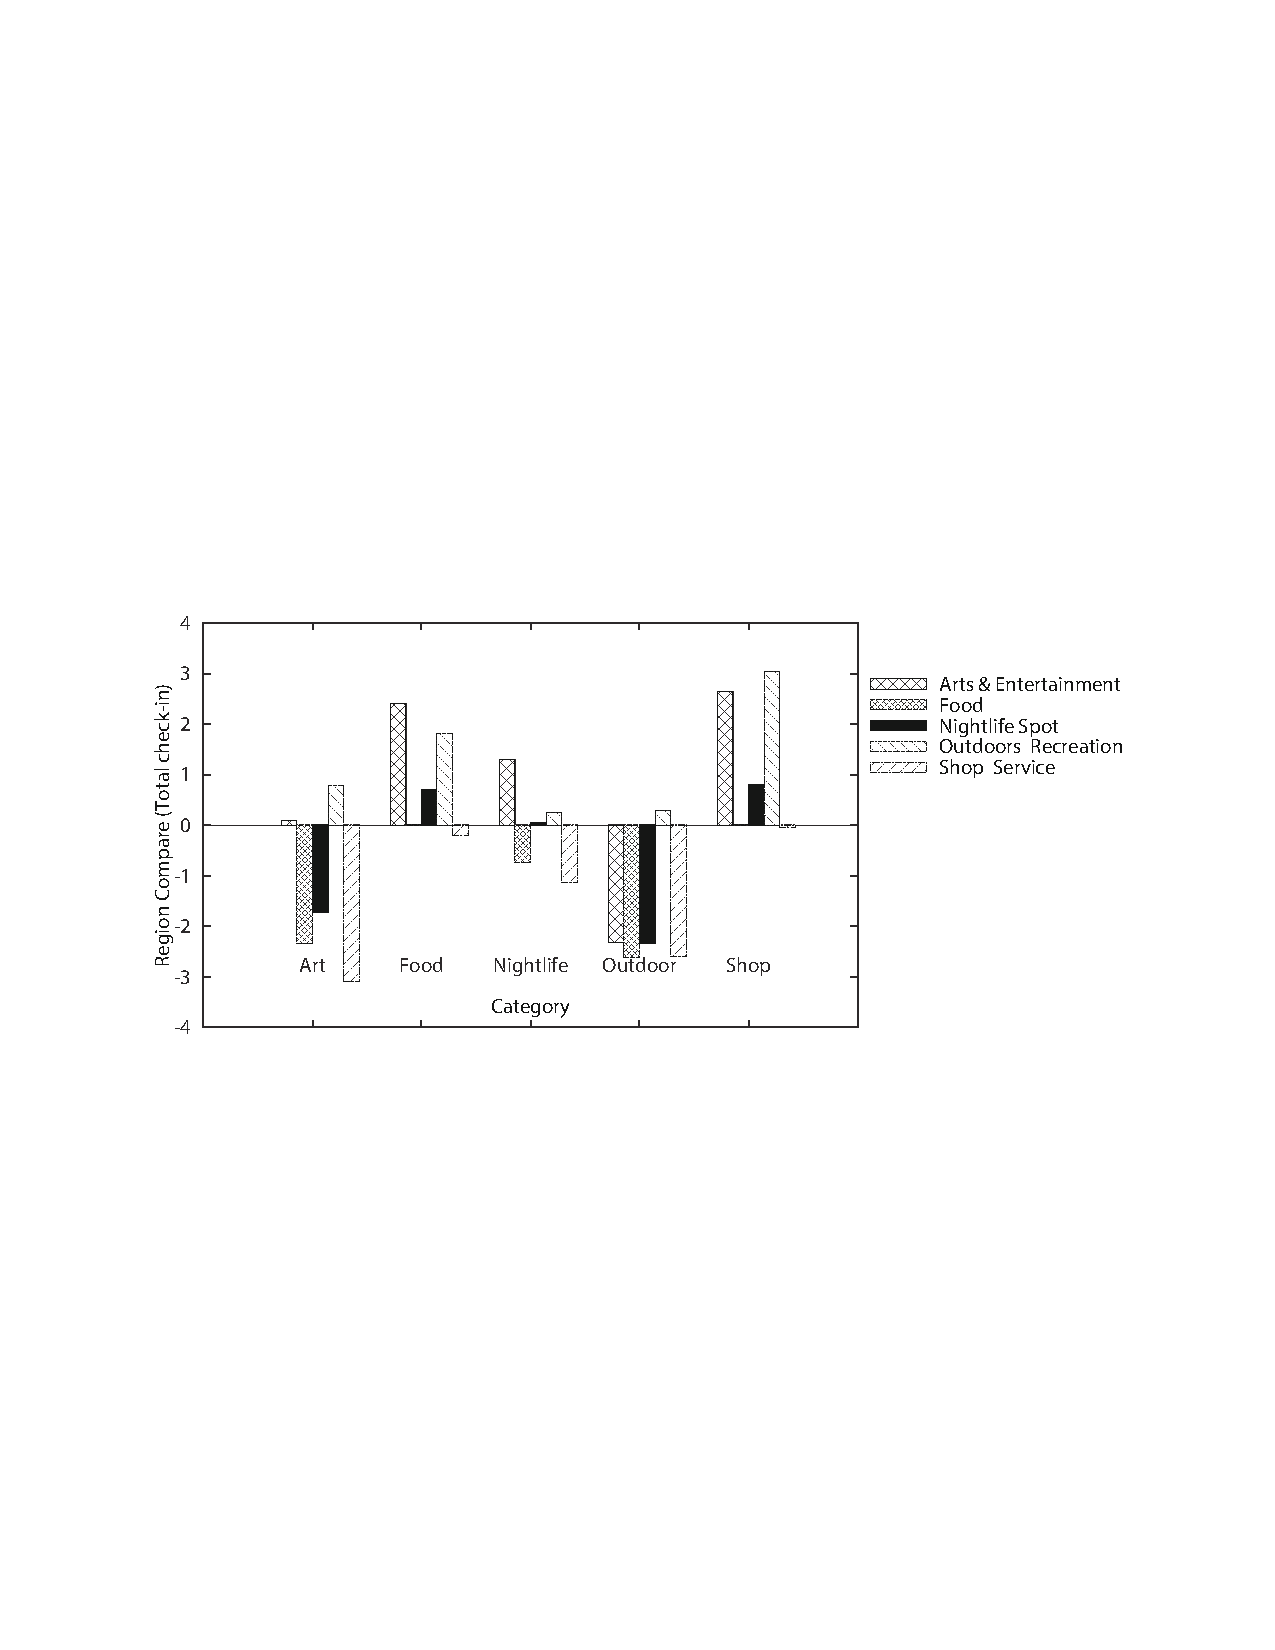
\epsfig{file=plot/RegionCompare.pdf,width=\columnwidth}
% figure caption is below the figure
\caption{Region Compare (Total Check-ins), score below 0 indicates more check-in time than other categories within same region}
\label{fig:RC}       % Give a unique label
\end{figure}
